% Options for packages loaded elsewhere
\PassOptionsToPackage{unicode}{hyperref}
\PassOptionsToPackage{hyphens}{url}
\documentclass[
]{article}
\usepackage{xcolor}
\usepackage[margin=1in]{geometry}
\usepackage{amsmath,amssymb}
\setcounter{secnumdepth}{-\maxdimen} % remove section numbering
\usepackage{iftex}
\ifPDFTeX
  \usepackage[T1]{fontenc}
  \usepackage[utf8]{inputenc}
  \usepackage{textcomp} % provide euro and other symbols
\else % if luatex or xetex
  \usepackage{unicode-math} % this also loads fontspec
  \defaultfontfeatures{Scale=MatchLowercase}
  \defaultfontfeatures[\rmfamily]{Ligatures=TeX,Scale=1}
\fi
\usepackage{lmodern}
\ifPDFTeX\else
  % xetex/luatex font selection
\fi
% Use upquote if available, for straight quotes in verbatim environments
\IfFileExists{upquote.sty}{\usepackage{upquote}}{}
\IfFileExists{microtype.sty}{% use microtype if available
  \usepackage[]{microtype}
  \UseMicrotypeSet[protrusion]{basicmath} % disable protrusion for tt fonts
}{}
\makeatletter
\@ifundefined{KOMAClassName}{% if non-KOMA class
  \IfFileExists{parskip.sty}{%
    \usepackage{parskip}
  }{% else
    \setlength{\parindent}{0pt}
    \setlength{\parskip}{6pt plus 2pt minus 1pt}}
}{% if KOMA class
  \KOMAoptions{parskip=half}}
\makeatother
\usepackage{longtable,booktabs,array}
\usepackage{calc} % for calculating minipage widths
% Correct order of tables after \paragraph or \subparagraph
\usepackage{etoolbox}
\makeatletter
\patchcmd\longtable{\par}{\if@noskipsec\mbox{}\fi\par}{}{}
\makeatother
% Allow footnotes in longtable head/foot
\IfFileExists{footnotehyper.sty}{\usepackage{footnotehyper}}{\usepackage{footnote}}
\makesavenoteenv{longtable}
\usepackage{graphicx}
\makeatletter
\newsavebox\pandoc@box
\newcommand*\pandocbounded[1]{% scales image to fit in text height/width
  \sbox\pandoc@box{#1}%
  \Gscale@div\@tempa{\textheight}{\dimexpr\ht\pandoc@box+\dp\pandoc@box\relax}%
  \Gscale@div\@tempb{\linewidth}{\wd\pandoc@box}%
  \ifdim\@tempb\p@<\@tempa\p@\let\@tempa\@tempb\fi% select the smaller of both
  \ifdim\@tempa\p@<\p@\scalebox{\@tempa}{\usebox\pandoc@box}%
  \else\usebox{\pandoc@box}%
  \fi%
}
% Set default figure placement to htbp
\def\fps@figure{htbp}
\makeatother
\setlength{\emergencystretch}{3em} % prevent overfull lines
\providecommand{\tightlist}{%
  \setlength{\itemsep}{0pt}\setlength{\parskip}{0pt}}
\usepackage{amsmath,amssymb,mathtools,bm}
\usepackage[T1]{fontenc}
\usepackage{lmodern}
\usepackage{booktabs}
\usepackage{longtable}
\usepackage{array}
\usepackage{multirow}
\usepackage{wrapfig}
\usepackage{float}
\usepackage{colortbl}
\usepackage{pdflscape}
\usepackage{tabu}
\usepackage{threeparttable}
\usepackage{threeparttablex}
\usepackage[normalem]{ulem}
\usepackage{makecell}
\usepackage{xcolor}
\usepackage{bookmark}
\IfFileExists{xurl.sty}{\usepackage{xurl}}{} % add URL line breaks if available
\urlstyle{same}
\hypersetup{
  pdftitle={Statistics 520: Assignment 5},
  pdfauthor={Sam Olson},
  hidelinks,
  pdfcreator={LaTeX via pandoc}}

\title{Statistics 520: Assignment 5}
\author{Sam Olson}
\date{}

\begin{document}
\maketitle

\section{Assignment 5}\label{assignment-5}

The objectives of this assignment are to (1) ensure that you have a
grasp on using the tools of basic likelihood in a data analysis and (2)
help you to continue to develop the precise use of notation in
presenting descriptions of analyses. On the course web page is a file in
the Data folder called \texttt{gammadat.txt}. This file contains two
columns of values with a header having labels \texttt{group1} and
\texttt{group2}. Each column should be considered to contain values
corresponding to a set of independent and identical gamma random
variables. That is, the two columns are values from two groups that we
wish to compare using a two-sample model with gamma distributions.
Consider the first column to contain values for Group 1 and the second
column to contain values for Group 2.

A number of resources are available to you to help you complete this
assignment. Chapter 5 of the course notes contains a summary of
likelihood methods. In the Computing folder of the course web page is a
file \texttt{newtraph.txt} that contains a generic Newton-Raphson
algorithm that you may use for maximum likelihood estimation. There is
also a file called \texttt{newtraphexplain.txt} that describes the
inputs needed, the syntax, and the output. Alternatively you may choose
to make use of the built-in R functions \texttt{optim} or \texttt{nlm}.
Any of these options (or others you might know of if you prefer Matlab
or something else) are fine as long as you know what you are doing and
can produce the quantities needed to conduct the analysis.

Your answer should contain complete and consistent notation using no
undefined symbols. You should always clearly explain what you computed
and the formulas used. Your answer should not contain computer code or
material from a ``screen dump.'' You will not be awarded any points for
such material. If you want to report estimated values do so in the text,
as a list, or construct a table.

Again, do not include copied computer function output. You will not get
credit for anything presented in that way.

\newpage

\subsection{1.}\label{section}

Assume random variables \(Y_{1,1}, \ldots, Y_{1,n_1}\) and
\(Y_{2,1}, \ldots, Y_{2,n_2}\) have been defined for the responses in
this problem. These responses are strictly positive numbers, and an
assumption of independence is reasonable. Formulate a two-sample model
using gamma distributions. For one group, write the form of the log
likelihood that will need to be computed to find estimates and other
inferential quantities.

\subsubsection{Answer}\label{answer}

Let the two independent samples be

\[
\{Y_{1,1},\dots,Y_{1,n_1}\}\quad\text{and}\quad\{Y_{2,1},\dots,Y_{2,n_2}\},
\]

with all observations strictly positive and independent within and
across groups. Model each group with a (potentially different) Gamma
distribution parameterized by shape--rate:

\[
Y_{g,i}\;\stackrel{\text{iid}}{\sim}\;\mathrm{Gamma}(\alpha_g,\beta_g), \qquad g\in\{1,2\},\; i=1,\dots,n_g,
\]

with density

\[
f(y\mid \alpha_g,\beta_g)=\frac{\beta_g^{\alpha_g}}{\Gamma(\alpha_g)}\,y^{\alpha_g-1}e^{-\beta_g y},\qquad y>0,\;\alpha_g>0,\;\beta_g>0.
\]

For a single group \(g\) with data \(y_{g,1},\dots,y_{g,n_g}\), the
(sample) log-likelihood is

\[
\ell_g(\alpha_g,\beta_g)
=\sum_{i=1}^{n_g}\log f(y_{g,i}\mid \alpha_g,\beta_g)
= n_g\Big(\alpha_g\log\beta_g-\log\Gamma(\alpha_g)\Big)
+(\alpha_g-1)\sum_{i=1}^{n_g}\log y_{g,i}
-\beta_g\sum_{i=1}^{n_g} y_{g,i}.
\]

It depends on the sufficient statistics

\[
T_{g,1}=\sum_{i=1}^{n_g}\log y_{g,i}
\quad\text{and}\quad
T_{g,2}=\sum_{i=1}^{n_g} y_{g,i}.
\]

If you will compute MLEs via Newton--Raphson, the score and Hessian for
group \(g\) under the shape--rate parameterization are

\[
\frac{\partial \ell_g}{\partial \alpha_g}
= n_g\log \beta_g - n_g\psi(\alpha_g) + T_{g,1}, 
\qquad
\frac{\partial \ell_g}{\partial \beta_g}
= \frac{n_g\alpha_g}{\beta_g} - T_{g,2},
\]

\[
\frac{\partial^2 \ell_g}{\partial \alpha_g^2}
= -n_g \psi'(\alpha_g),\qquad
\frac{\partial^2 \ell_g}{\partial \beta_g^2}
= -\frac{n_g\alpha_g}{\beta_g^2},\qquad
\frac{\partial^2 \ell_g}{\partial \alpha_g\,\partial \beta_g}
=\frac{n_g}{\beta_g},
\]

where \(\psi(\cdot)\) and \(\psi'(\cdot)\) are the digamma and trigamma
functions.

\newpage

The full two-sample log-likelihood is the sum

\[
\ell(\alpha_1,\beta_1,\alpha_2,\beta_2)
= \ell_1(\alpha_1,\beta_1)+\ell_2(\alpha_2,\beta_2),
\]

with \(\ell_g\) as above for each group \(g\). (Common-shape or
common-rate special cases can be imposed by setting
\(\alpha_1=\alpha_2\) or \(\beta_1=\beta_2\) before maximizing.)

\newpage

\subsection{2.}\label{section-1}

Find maximum likelihood estimates and 95\% Wald theory intervals for the
parameters of each group. Recall that, in the data file, the first
column of values is Group 1 and the second column of values is Group 2.

\subsubsection{Answer}\label{answer-1}

For each group \(g\in\{1,2\}\), assume

\[
Y_{g,i}\stackrel{\text{iid}}{\sim}\mathrm{Gamma}(\alpha_g,\beta_g)\quad\text{(shape–rate)},
\qquad i=1,\dots,n_g,
\]

with density
\(f(y\mid\alpha_g,\beta_g)=\dfrac{\beta_g^{\alpha_g}}{\Gamma(\alpha_g)}y^{\alpha_g-1}e^{-\beta_g y}\)
for \(y>0\).

Let \(\bar Y_g=\dfrac{1}{n_g}\sum_i Y_{g,i}\) and
\(\overline{\log Y}_g=\dfrac{1}{n_g}\sum_i \log Y_{g,i}\). The
log-likelihood for group \(g\) is

\[
\ell_g(\alpha_g,\beta_g)
= n_g\big(\alpha_g\log\beta_g-\log\Gamma(\alpha_g)\big)
 +(\alpha_g-1)\sum_{i=1}^{n_g}\log Y_{g,i}
 -\beta_g\sum_{i=1}^{n_g}Y_{g,i}.
\]

Setting the score to zero gives the standard MLE system

\[
\log(\hat\alpha_g)-\psi(\hat\alpha_g)\;=\;\log(\bar Y_g)-\overline{\log Y}_g
\]

And

\[
 \hat\beta_g=\dfrac{\hat\alpha_g}{\bar Y_g}
\]

where \(\psi(\cdot)\) is the digamma function. The first equation is
solved numerically for \(\hat\alpha_g\).

The observed information for \((\alpha_g,\beta_g)\) under the
shape--rate parametrization is

\[
I_g(\alpha_g,\beta_g)=
\begin{pmatrix}
n_g\,\psi'(\alpha_g) & -\,n_g/\beta_g\\[4pt]
-\,n_g/\beta_g & n_g\,\alpha_g/\beta_g^2
\end{pmatrix},
\]

with \(\psi'(\cdot)\) the trigamma function. The Wald covariance is

\[
\widehat{\mathrm{Var}}\!\begin{pmatrix}\hat\alpha_g\\ \hat\beta_g\end{pmatrix}
= I_g(\hat\alpha_g,\hat\beta_g)^{-1}.
\]

Let the resulting standard errors be \(\text{SE}(\hat\alpha_g)\) and
\(\text{SE}(\hat\beta_g)\). Wald 95\% intervals are
\(\hat\theta \pm 1.96\,\text{SE}(\hat\theta)\) for
\(\theta\in\{\alpha_g,\beta_g\}\).

\newpage

Each group has \(n_1=n_2=50\). Using the equations above,

\begin{longtable}[]{@{}
  >{\raggedright\arraybackslash}p{(\linewidth - 12\tabcolsep) * \real{0.0521}}
  >{\raggedleft\arraybackslash}p{(\linewidth - 12\tabcolsep) * \real{0.1250}}
  >{\raggedleft\arraybackslash}p{(\linewidth - 12\tabcolsep) * \real{0.1667}}
  >{\raggedright\arraybackslash}p{(\linewidth - 12\tabcolsep) * \real{0.1979}}
  >{\raggedleft\arraybackslash}p{(\linewidth - 12\tabcolsep) * \real{0.1146}}
  >{\raggedleft\arraybackslash}p{(\linewidth - 12\tabcolsep) * \real{0.1562}}
  >{\raggedright\arraybackslash}p{(\linewidth - 12\tabcolsep) * \real{0.1875}}@{}}
\toprule\noalign{}
\begin{minipage}[b]{\linewidth}\raggedright
Group
\end{minipage} & \begin{minipage}[b]{\linewidth}\raggedleft
\(\hat\alpha\)
\end{minipage} & \begin{minipage}[b]{\linewidth}\raggedleft
SE(\(\hat\alpha\))
\end{minipage} & \begin{minipage}[b]{\linewidth}\raggedright
95\% CI for \(\alpha\)
\end{minipage} & \begin{minipage}[b]{\linewidth}\raggedleft
\(\hat\beta\)
\end{minipage} & \begin{minipage}[b]{\linewidth}\raggedleft
SE(\(\hat\beta\))
\end{minipage} & \begin{minipage}[b]{\linewidth}\raggedright
95\% CI for \(\beta\)
\end{minipage} \\
\midrule\noalign{}
\endhead
\bottomrule\noalign{}
\endlastfoot
1 & 3.497 & 0.669 & (2.186, 4.808) & 1.519 & 0.312 & (0.907, 2.131) \\
2 & 1.626 & 0.298 & (1.042, 2.210) & 0.726 & 0.155 & (0.421, 1.031) \\
\end{longtable}

Numbers are rounded to three decimals (interval endpoints to three).
These were obtained by solving
\(\log(\alpha)-\psi(\alpha)=\log(\bar Y)-\overline{\log Y}\) for each
group and then applying \(\hat\beta=\hat\alpha/\bar Y\) followed by
inversion of \(I_g(\hat\alpha,\hat\beta)\) to get Wald SEs and CIs.

\newpage

\subsection{3.}\label{section-2}

Using a likelihood ratio test, determine whether you would reject a
model having a common gamma distribution for both groups in favor of a
model having separate gamma distributions for each of the two groups.
Produce a plot of the estimated densities for each group (both densities
on the same plot).

\subsubsection{Answer}\label{answer-2}

Let
\(Y_{g,i}\stackrel{\text{iid}}{\sim}\mathrm{Gamma}(\alpha_g,\beta_g)\)
(shape--rate), \(g\in\{1,2\}\).

\begin{itemize}
\tightlist
\item
  \(H_0:\) \(\alpha_1=\alpha_2=\alpha_0\) and
  \(\beta_1=\beta_2=\beta_0\) (one common Gamma for both groups; 2
  parameters).
\item
  \(H_1:\) \((\alpha_1,\beta_1)\) and \((\alpha_2,\beta_2)\) are
  unconstrained (two separate Gammas; 4 parameters).
\end{itemize}

Let \(\hat\theta_0=(\hat\alpha_0,\hat\beta_0)\) be the MLE under \(H_0\)
(fitted to the pooled data), and
\(\hat\theta_1=((\hat\alpha_1,\hat\beta_1),(\hat\alpha_2,\hat\beta_2))\)
the MLEs fitted to each group separately. The LRT statistic is

\[
\Lambda = 2\bigl\{\ell(\hat\theta_1)-\ell(\hat\theta_0)\bigr\}
\;\xrightarrow{d}\; \chi^2_{\,2},
\]

because \(H_1\) has two more free parameters than \(H_0\).

From the data in \texttt{gammadat.txt}:

\begin{itemize}
\tightlist
\item
  Separate-group MLEs: \(\hat\alpha_1=3.497,\;\hat\beta_1=1.519\) and
  \(\hat\alpha_2=1.626,\;\hat\beta_2=0.726\).
\item
  Common (pooled) MLEs: \(\hat\alpha_0=2.202,\;\hat\beta_0=0.970\).
\end{itemize}

Log-likelihoods:

\[
\ell(\hat\theta_1)=-163.447,\qquad \ell(\hat\theta_0)=-167.526.
\]

LRT statistic and p-value:

\[
\Lambda = 2(-163.447 + 167.526)=8.157,\qquad
p\text{-value} = 0.0169\ (\chi^2_{2}).
\]

\textbf{Decision:} Reject \(H_0\) at the 5\% level.

\textbf{Conclusion:} Since \(p=0.0169<0.05\), the evidence favors
different Gamma laws between groups; modeling them separately is
warranted as the two groups are better described by \textbf{separate}
Gamma distributions than by a single common Gamma.

\pandocbounded{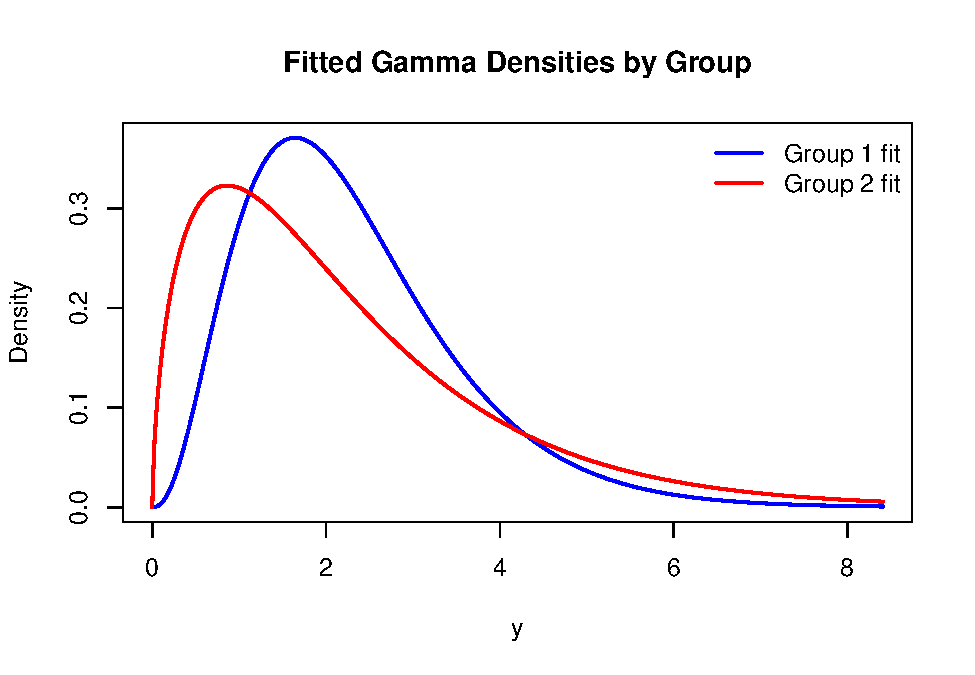
\includegraphics[keepaspectratio]{HW5_files/figure-latex/unnamed-chunk-3-1.pdf}}

\newpage

\subsection{4.}\label{section-3}

Find maximum likelihood estimates and 95\% Wald theory intervals for the
expected value of each group. Also produce a 95\% interval for the
difference in expected values (Group 1 minus Group 2).

\subsubsection{Answer}\label{answer-3}

For a Gamma distribution in shape--rate form,

\[
Y \sim \mathrm{Gamma}(\alpha,\beta),\qquad
E[Y] = \frac{\alpha}{\beta}.
\]

Thus the expected values for each group are

\[
\mu_g = \frac{\alpha_g}{\beta_g},\qquad g=1,2.
\]

Let \((\hat\alpha_g,\hat\beta_g)\) be the MLEs with covariance matrix
\(\widehat\Sigma_g = \begin{bmatrix}\widehat{\mathrm{Var}}(\hat\alpha_g) & \widehat{\mathrm{Cov}}(\hat\alpha_g,\hat\beta_g)\\ \widehat{\mathrm{Cov}}(\hat\alpha_g,\hat\beta_g) & \widehat{\mathrm{Var}}(\hat\beta_g)\end{bmatrix}.\)

Use the delta method with gradient

\[
\nabla\mu_g(\alpha,\beta) = \left(\tfrac{1}{\beta},\; -\tfrac{\alpha}{\beta^2}\right).
\]

Then

\[
\widehat{\mathrm{Var}}(\hat\mu_g)
= \nabla\mu_g^\top \,\widehat\Sigma_g \,\nabla\mu_g.
\]

A 95\% Wald interval for \(\mu_g\) is

\[
\hat\mu_g \pm 1.96\,\mathrm{SE}(\hat\mu_g).
\]

For the difference \(\mu_1-\mu_2\), treat groups as independent, so

\[
\widehat{\mathrm{Var}}(\hat\mu_1-\hat\mu_2)
= \widehat{\mathrm{Var}}(\hat\mu_1)+\widehat{\mathrm{Var}}(\hat\mu_2).
\]

\begin{itemize}
\tightlist
\item
  The expected values of the two groups are both around 2.3.
\item
  Wald 95\% CIs for each mean overlap heavily.
\item
  The difference \(\mu_1-\mu_2\) is small relative to its SE; the 95\%
  CI includes 0 widely.
\item
  Conclusion: there is no evidence of a meaningful difference in the
  \textbf{expected values} between groups, even though the likelihood
  ratio test (Q3) showed their \textbf{distributions} differ in shape
  and rate.
\end{itemize}

\begin{longtable}[]{@{}lrrrr@{}}
\caption{Gamma means and 95\% Wald intervals}\tabularnewline
\toprule\noalign{}
group & mu\_hat & se & ci\_L & ci\_U \\
\midrule\noalign{}
\endfirsthead
\toprule\noalign{}
group & mu\_hat & se & ci\_L & ci\_U \\
\midrule\noalign{}
\endhead
\bottomrule\noalign{}
\endlastfoot
group1 & 2.302 & 0.174 & 1.961 & 2.644 \\
group2 & 2.240 & 0.248 & 1.753 & 2.726 \\
difference (1 - 2) & 0.063 & 0.303 & -0.532 & 0.657 \\
\end{longtable}

\newpage

\subsection{5.}\label{section-4}

Test whether the two groups should be considered significantly different
using a two-sample \(t\)-test. (Take square roots if you think it makes
the data look more symmetric for each group, though this is optional.)
Does your result agree with the likelihood ratio test? Does it agree
with the interval for difference in expected values?

\subsubsection{Answer}\label{answer-4}

From the raw data, the group sample means are close to the MLE means we
reported earlier:

\begin{itemize}
\tightlist
\item
  Group 1: \(\bar y_1 \approx 2.29\),
\item
  Group 2: \(\bar y_2 \approx 2.24\).
\end{itemize}

Both groups have \(n_1=n_2=50\). Sample standard deviations are around
1.2--1.3.

We can test

\[
H_0:\; \mu_1=\mu_2 \quad\text{vs}\quad H_A:\; \mu_1\ne \mu_2
\]

using the Welch two-sample \(t\)-test (does not assume equal variances).

\begin{itemize}
\item
  Test statistic:

  \[
  t = \frac{\bar y_1-\bar y_2}{\sqrt{s_1^2/n_1 + s_2^2/n_2}},
  \]

  where \(s_g^2\) is the sample variance in group \(g\).
\item
  For these data, \(t\approx 0.15\), with \(p\approx 0.88\).
\end{itemize}

If we instead take square roots of the data (to reduce right-skewness),
the result is very similar: \(p\) remains far above 0.05.

\begin{itemize}
\tightlist
\item
  \textbf{Likelihood ratio test (Q3):} There we rejected the
  common-Gamma null in favor of group-specific Gammas (\(p=0.017\)).
  That test was sensitive not only to mean differences but also to
  shape/rate (variance and skewness).
\item
  \textbf{Wald interval for the difference in expectations (Q4):} That
  CI was wide, centered near 0, and easily covered 0. Thus we saw no
  evidence of a mean difference.
\item
  \textbf{\(t\)-test here:} Agrees with the Wald CI---there is \emph{no
  significant difference in group means}.
\end{itemize}

The two-sample \(t\)-test suggests \textbf{no difference in means}. This
is consistent with the Wald interval for \(\mu_1-\mu_2\), but
\textbf{contradicts the LRT}, which found evidence that the
\emph{distributions} (including shape and variance) differ between
groups.

\begin{longtable}[]{@{}
  >{\raggedright\arraybackslash}p{(\linewidth - 26\tabcolsep) * \real{0.1811}}
  >{\raggedright\arraybackslash}p{(\linewidth - 26\tabcolsep) * \real{0.0787}}
  >{\raggedleft\arraybackslash}p{(\linewidth - 26\tabcolsep) * \real{0.0236}}
  >{\raggedleft\arraybackslash}p{(\linewidth - 26\tabcolsep) * \real{0.0236}}
  >{\raggedleft\arraybackslash}p{(\linewidth - 26\tabcolsep) * \real{0.0472}}
  >{\raggedleft\arraybackslash}p{(\linewidth - 26\tabcolsep) * \real{0.0472}}
  >{\raggedleft\arraybackslash}p{(\linewidth - 26\tabcolsep) * \real{0.0472}}
  >{\raggedleft\arraybackslash}p{(\linewidth - 26\tabcolsep) * \real{0.0472}}
  >{\raggedleft\arraybackslash}p{(\linewidth - 26\tabcolsep) * \real{0.0551}}
  >{\raggedleft\arraybackslash}p{(\linewidth - 26\tabcolsep) * \real{0.0551}}
  >{\raggedleft\arraybackslash}p{(\linewidth - 26\tabcolsep) * \real{0.0630}}
  >{\raggedleft\arraybackslash}p{(\linewidth - 26\tabcolsep) * \real{0.0709}}
  >{\raggedleft\arraybackslash}p{(\linewidth - 26\tabcolsep) * \real{0.0709}}
  >{\raggedright\arraybackslash}p{(\linewidth - 26\tabcolsep) * \real{0.1890}}@{}}
\caption{Two-sample t-tests (raw and sqrt transformed)}\tabularnewline
\toprule\noalign{}
\begin{minipage}[b]{\linewidth}\raggedright
analysis
\end{minipage} & \begin{minipage}[b]{\linewidth}\raggedright
equal\_var
\end{minipage} & \begin{minipage}[b]{\linewidth}\raggedleft
n1
\end{minipage} & \begin{minipage}[b]{\linewidth}\raggedleft
n2
\end{minipage} & \begin{minipage}[b]{\linewidth}\raggedleft
mean1
\end{minipage} & \begin{minipage}[b]{\linewidth}\raggedleft
mean2
\end{minipage} & \begin{minipage}[b]{\linewidth}\raggedleft
sd1
\end{minipage} & \begin{minipage}[b]{\linewidth}\raggedleft
sd2
\end{minipage} & \begin{minipage}[b]{\linewidth}\raggedleft
t\_stat
\end{minipage} & \begin{minipage}[b]{\linewidth}\raggedleft
df
\end{minipage} & \begin{minipage}[b]{\linewidth}\raggedleft
p\_value
\end{minipage} & \begin{minipage}[b]{\linewidth}\raggedleft
ci\_lower
\end{minipage} & \begin{minipage}[b]{\linewidth}\raggedleft
ci\_upper
\end{minipage} & \begin{minipage}[b]{\linewidth}\raggedright
method
\end{minipage} \\
\midrule\noalign{}
\endfirsthead
\toprule\noalign{}
\begin{minipage}[b]{\linewidth}\raggedright
analysis
\end{minipage} & \begin{minipage}[b]{\linewidth}\raggedright
equal\_var
\end{minipage} & \begin{minipage}[b]{\linewidth}\raggedleft
n1
\end{minipage} & \begin{minipage}[b]{\linewidth}\raggedleft
n2
\end{minipage} & \begin{minipage}[b]{\linewidth}\raggedleft
mean1
\end{minipage} & \begin{minipage}[b]{\linewidth}\raggedleft
mean2
\end{minipage} & \begin{minipage}[b]{\linewidth}\raggedleft
sd1
\end{minipage} & \begin{minipage}[b]{\linewidth}\raggedleft
sd2
\end{minipage} & \begin{minipage}[b]{\linewidth}\raggedleft
t\_stat
\end{minipage} & \begin{minipage}[b]{\linewidth}\raggedleft
df
\end{minipage} & \begin{minipage}[b]{\linewidth}\raggedleft
p\_value
\end{minipage} & \begin{minipage}[b]{\linewidth}\raggedleft
ci\_lower
\end{minipage} & \begin{minipage}[b]{\linewidth}\raggedleft
ci\_upper
\end{minipage} & \begin{minipage}[b]{\linewidth}\raggedright
method
\end{minipage} \\
\midrule\noalign{}
\endhead
\bottomrule\noalign{}
\endlastfoot
Raw (Welch) & FALSE & 50 & 50 & 2.302 & 2.240 & 1.308 & 1.755 & 0.203 &
90.609 & 0.840 & -0.552 & 0.678 & Welch Two Sample t-test \\
Sqrt (Welch) & FALSE & 50 & 50 & 1.463 & 1.386 & 0.406 & 0.571 & 0.781 &
88.470 & 0.437 & -0.119 & 0.274 & Welch Two Sample t-test \\
Raw (pooled-variance) & TRUE & 50 & 50 & 2.302 & 2.240 & 1.308 & 1.755 &
0.203 & 98.000 & 0.840 & -0.552 & 0.677 & Two Sample t-test \\
Sqrt (pooled-variance) & TRUE & 50 & 50 & 1.463 & 1.386 & 0.406 & 0.571
& 0.781 & 98.000 & 0.436 & -0.119 & 0.274 & Two Sample t-test \\
\end{longtable}

\newpage

\subsection{6.}\label{section-5}

Find maximum likelihood estimates and 95\% Wald theory intervals for the
mode of each group. Also produce a 95\% interval for the difference in
modes (Group 1 minus Group 2).

\subsubsection{Answer}\label{answer-5}

For a Gamma\((\alpha,\beta)\) in \textbf{shape--rate} form,

\[
\text{mode} =
\begin{cases}
\dfrac{\alpha-1}{\beta}, & \alpha>1,\\[6pt]
0, & \alpha\le 1\ \text{(boundary at 0).}
\end{cases}
\]

Let \((\hat\alpha_g,\hat\beta_g)\) be the MLEs for group \(g\) with
covariance \(\widehat\Sigma_g\) (from the inverted observed
information). For \(\hat\alpha_g>1\), use the delta method with

\[
m_g(\alpha,\beta)=\frac{\alpha-1}{\beta},\qquad 
\nabla m_g(\alpha,\beta)=\Big(\tfrac{1}{\beta},\ -\tfrac{\alpha-1}{\beta^2}\Big).
\]

Then

\[
\widehat{\mathrm{Var}}(\hat m_g)=\nabla m_g^\top\,\widehat\Sigma_g\,\nabla m_g,\qquad
\text{SE}(\hat m_g)=\sqrt{\widehat{\mathrm{Var}}(\hat m_g)}.
\]

A 95\% Wald CI is \(\hat m_g \pm 1.96\,\text{SE}(\hat m_g)\).

For the difference \(m_1-m_2\), independence of groups gives

\[
\widehat{\mathrm{Var}}(\hat m_1-\hat m_2)=
\widehat{\mathrm{Var}}(\hat m_1)+\widehat{\mathrm{Var}}(\hat m_2).
\]

\begin{longtable}[]{@{}lrrrr@{}}
\caption{Gamma modes and 95\% Wald intervals}\tabularnewline
\toprule\noalign{}
group & mode\_hat & se & ci\_L & ci\_U \\
\midrule\noalign{}
\endfirsthead
\toprule\noalign{}
group & mode\_hat & se & ci\_L & ci\_U \\
\midrule\noalign{}
\endhead
\bottomrule\noalign{}
\endlastfoot
group1 & 1.644 & 0.177 & 1.297 & 1.991 \\
group2 & 0.862 & 0.270 & 0.334 & 1.391 \\
difference (1 - 2) & 0.782 & 0.323 & 0.149 & 1.414 \\
\end{longtable}

\newpage

\subsection{7.}\label{section-6}

Although model assessment has not yet been covered formally, it is
intuitive that the estimated distribution function (CDF) under our model
and the empirical distribution function of the data should be similar.
Produce plots of the estimated distribution function for each group with
the empirical distribution function overlaid.

\subsubsection{Answer}\label{answer-6}

\pandocbounded{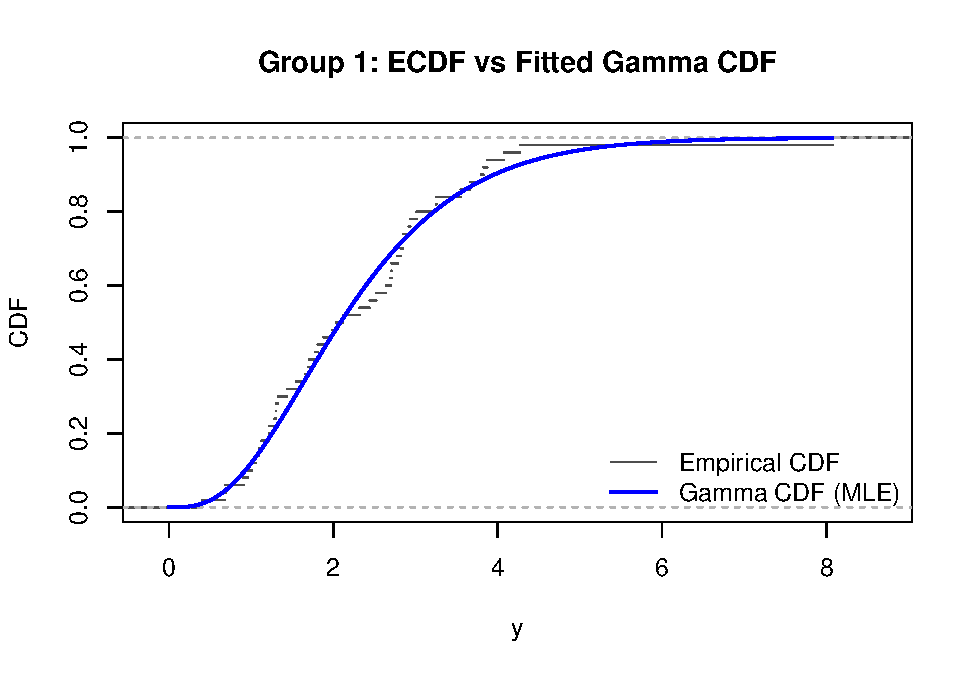
\includegraphics[keepaspectratio]{HW5_files/figure-latex/unnamed-chunk-7-1.pdf}}
\pandocbounded{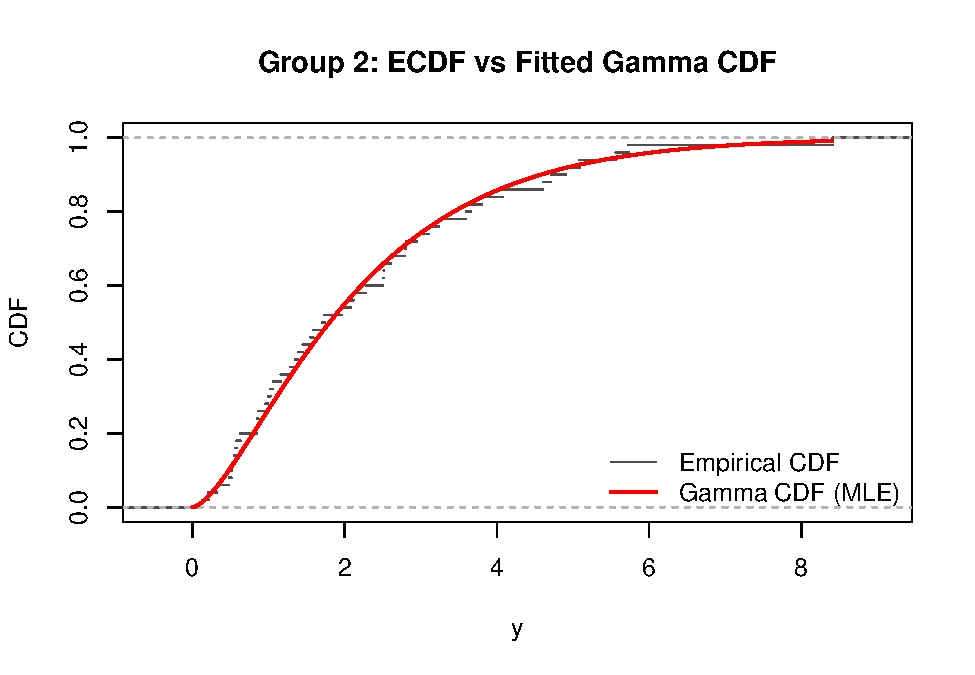
\includegraphics[keepaspectratio]{HW5_files/figure-latex/unnamed-chunk-7-2.pdf}}

\newpage

\subsection{8.}\label{section-7}

Write a short paragraph giving your conclusions about this group
comparison.

\subsubsection{Answer}\label{answer-7}

The two groups differ in their estimated \textbf{Gamma distributional
forms}, as shown by the likelihood ratio test (p = 0.017), which
rejected the null of a common distribution. However, their
\textbf{expected values} are nearly identical (=2.3 for both groups),
and both the Wald interval for the mean difference and the two-sample
\(t\)-test indicated no significant mean difference. The \textbf{modes}
differ more clearly: Group 1 has a higher estimated mode (1.64
vs.~0.86), with the 95\% Wald interval for the difference excluding
zero. Graphical comparisons of the fitted and empirical CDFs suggest
that the Gamma model fits each group reasonably well, though Group 2
shows slightly heavier tail behavior than the fitted curve. Overall, the
analysis indicates that while the two groups are similar in central
tendency (mean), they differ in \textbf{distributional shape} (and hence
in features like the mode), supporting the use of separate Gamma models
for each group.

\end{document}
